In a recent years wide cloud adoption has coused huge momentum in adopting software architecture known as micro-services, as it is a native architecture for the cloud. This project will also adapt this architecture because part of the deployment is being done in cloud, and swarm of agents can also be simulated using this approach. Moreover technologies such as kind and tilt made it easier to develop all services locally using local kubernetes cluster.

{\color{red}What are microservices?}

\begin{figure}[H]
    \centering
    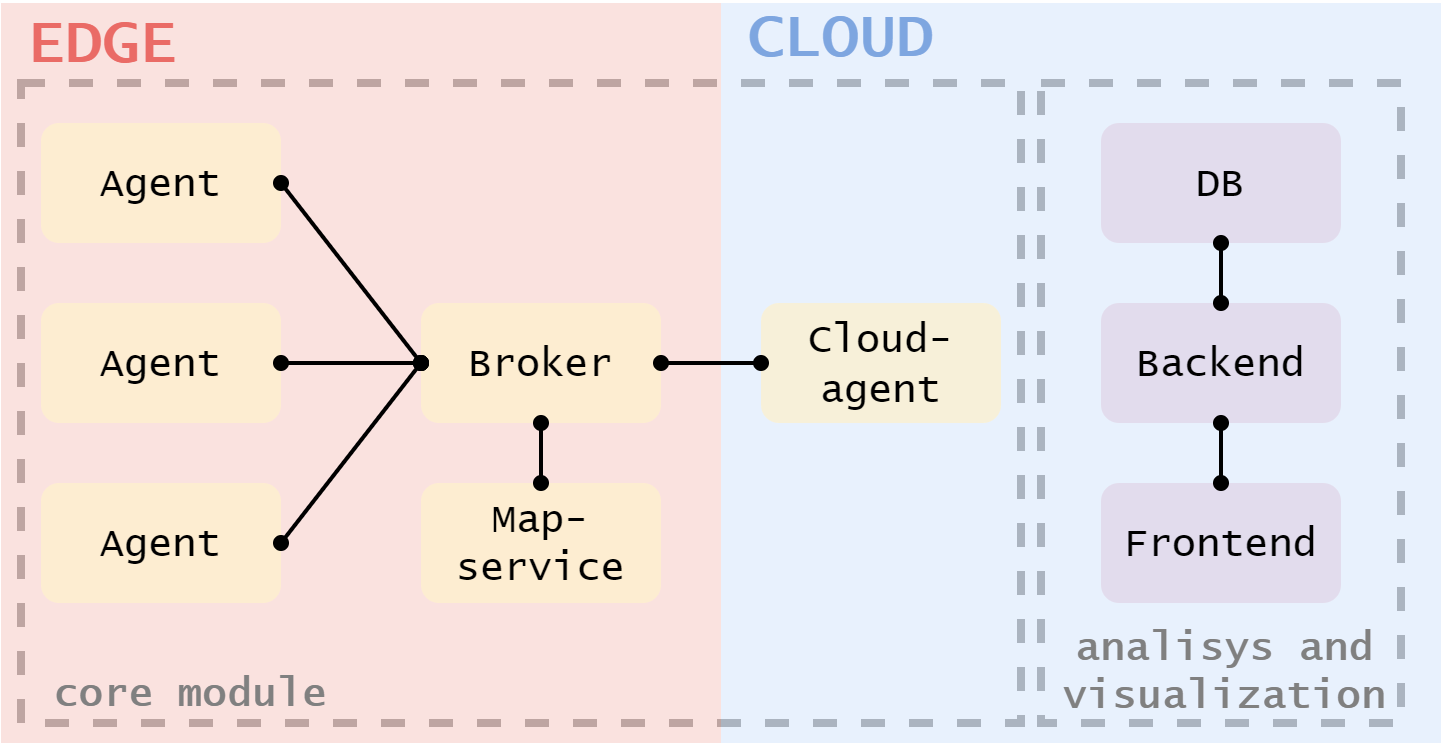
\includegraphics[width=\textwidth]{pictures/services.png}
    \caption{ Micro services system design }
    \label{fig:micro_services}
\end{figure}

\subsection{Agent}
{\color{red}What time should i use(will, is, was)?}
Agent is a microservice which is implementing the logic of the entity which needs to plan a path.  It is meant to have limited resources to simulate real world scenario, and number of its instances will vary.

When agent is started, it doesn't belong to any swarm so it will start local discovery to find his peers. After peers are found, one of the agent has to be elected as a leader and therefore election algorithm will be initiated in on e or multiple agent and on agent will be elected to be a swarm leader. Agent will periodically poll his peers to check their liveness and it this behaviour will be refereed as liveness check.

This entity contain also all algorithms meant for path planning as in a base case scenario, computation will take place in the agent to obtain path.

\subsection{Cloud-agent}
Cloud-agent is an entity to which computation can be upstream to offload the agents. It will have much more computing power, but it might be located in different geographically location so latency between local agents and this one will matter in case of total calculation time.

This microservice will be deployed in the cloud and it will use cloud-broker as a communication medium.

\subsection{Broker}
Service responsible of communication between the services. It will be deployed both in cloud and in the local environment, and those two entities should be connected with a bridge. This will be a single connection point between cloud and edge.

{\color{red}Maybe explain in mqtt part)?}
This entity will use pub/sub approach to handle and distribute the messages.

\subsection{Map-service}
Initially when agents are spawned they do not have any map assigned. After electing a leader he will trigger new map generation, by message passing to map-service. This entity is responsible of creation the map and spawning agent in it. It is a substitute of sensing for the agent as it gives the robots all information they need for finding in position in a global map.

Additionally pre-defined map are stored in this service and can be adopted by the agent upon specific query. Note that map-service can spawn agent in a places wher it is not possible to reach the goal, but it is also a valid scenario.

\subsection{Backend}
It is a service meant for gathering data and interacting with a core module(agent, map-service etc.). It exposes endpoint throug REST api(endpoints in the appendix A) and forwards request to MQTT broker. It is also receiving data from alll the entities and stores it in a database connected to it. Backend is deployed in a cloud and it connects to a cloud-broker, endpoints should be exposed to the end-user.

\subsection{Frontend}
End user gragphical interface, deployed as a web-service is called frontend. It is taking inputs from the user and triggering specific actions through backend service API. It is also used for raw data visualization and it is deployed in a cloud and exposed to end user. It's capabilities are explained in \hyperref[sec:0308]{visualization section} of this chapter.